\documentclass{article}
\usepackage[utf8]{inputenc}
\usepackage{graphicx}
\usepackage[section]{placeins}
\usepackage{booktabs}
\usepackage[export]{adjustbox}
\usepackage[a4paper, margin=2cm]{geometry}
\usepackage{subfig}


\title{Traffic stops at Rhode Island}
\author{Laura Barranco Navarro }
\date{February 2022}

\begin{document}

\maketitle
\newpage
\tableofcontents
\newpage
\section{Introduction}
This project uses data from "The Stanford open policing  project"~\cite{StanfordWeb,StanfordPaper} to analyse traffic stops by police officers in the Rhode Island State of the United States. After cleaning the data, several questions are answered by analysing it and by using visualisation tools. In particular, we are interested in analysing the impact of gender  on the stops patterns. We also look at the different patterns over time. 

In addition, we combine this dataset with weather information from the "National Centers for Environmental Information"~\cite{WeatherWeb} to understand if the weather conditions have an impact on the police stops patterns.

This project is inspired by the DataCamp project~\cite{DataCamp}. 

\section{The data}

\begin{itemize}
\item Traffic stops data correspond to 509,671 stops during the period January 2005 to December 2015 in the Rhode Island state. It is taken from the "The Stanford open policing project"\cite{StanfordWeb}.

\item Weather data from the PROVIDENCE, RI US station corresponding to the period October 1942 to December 2021. It is taken from the "National Centers for Environmental Information"\cite{WeatherWeb}.

\end{itemize}

\section{Studies by gender}

The dataset stores information about the reason for the stop (speeding,  equipment/inspection violation, motorist assist/courtesy,  registration violation, call for service, 
 violation of city/town ordinance, special detail/directed patrol, APB, warrant, suspicious person, seatbelt violation, other traffic violation), the outcome of the stop (citation, warning, arrest) or if a search was performed, among others. This section looks at these variables in terms of the gender of the conductor. 
 
  \begin{figure}[h]
\subfloat[]{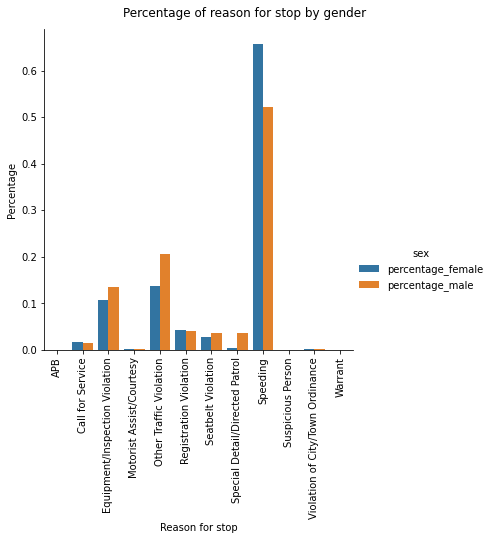
\includegraphics[scale=0.34, valign=t]{../figures/reason_gender.png}}
\subfloat[]{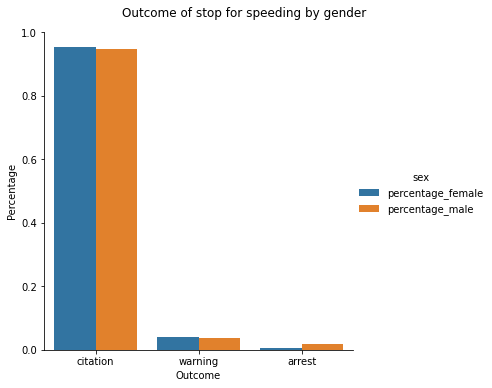
\includegraphics[scale=0.34, valign=t]{../figures/speeding_outcome_gender.png}}
\subfloat[]{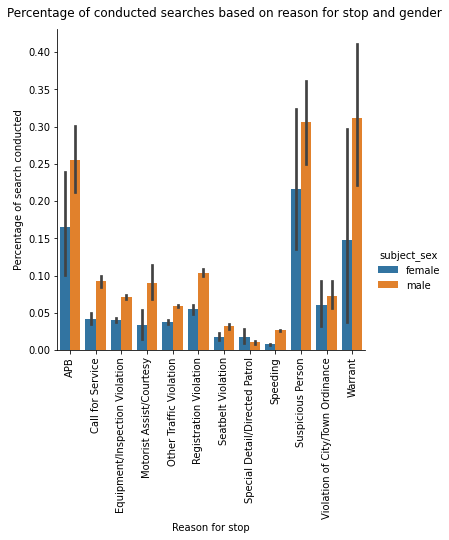
\includegraphics[scale=0.34, valign=t]{../figures/search_reason_gender.png}}
\caption{Frequency of: reason for stop (a), outcome of stops due to speeding (b) and search rate per reason for stop (c) split by the gender of the conductor.} \label{gender_studies}
\end{figure}   
 
Figure~\ref{gender_studies} shows the frequency of these variables. Figure\ref{gender_studies}~(a) depicts the frequency of the different reasons for stop. We observe that the main reason is speeding: 65.7\% in the case of females and 52.2\% in the case of males. These numbers can be read as well in Table~\ref{tab:reason}. Speeding is followed by other traffic violations and equipment/inspection violation. Even though speeding is by far the main reason in both genders, we see the difference is even bigger in the case of females. 

Figure~\ref{gender_studies}~(b) and Table~\ref{tab:outcome} show the outcome of the stop for the stops due to the speeding violation.  Around 95\% of the stops result in a citation and no significant differences are observed according to the gender.

Finally, Figure~\ref{gender_studies}~(c) shows how often a search is performed according to the reason for the stop and the gender of the driver. Numbers can be read in Table~\ref{tab:search}. As a general trend, male drivers get searched more often that female drivers. Conductors are searched more frequently when there is a warrant, an APB\footnote{All Points Bulletin: a broadcast alert from one police station to all others in an area, state, etc., as with instructions to arrest a particular suspect or suspects.} or if the driver looks suspicious.


\FloatBarrier


\begin{table}[htbp]
\begin{center}
\begin{tabular}{lrr}
\toprule
                  Reason for stop & Female & Male \\
\midrule
                        Speeding &  0.657 & 0.522 \\
         Other Traffic Violation &  0.137 & 0.207 \\
  Equipment/Inspection Violation &  0.107 & 0.135 \\
          Registration Violation &  0.043 & 0.041 \\
              Seatbelt Violation &  0.027 & 0.037 \\
                Call for Service &  0.018 & 0.015 \\
  Special Detail/Directed Patrol &  0.005 & 0.037 \\
        Motorist Assist/Courtesy &  0.003 & 0.002 \\
Violation of City/Town Ordinance &  0.002 & 0.002 \\
                             APB &  0.001 & 0.001 \\
               Suspicious Person &  0.001 & 0.001 \\
                         Warrant &  0.000 & 0.000 \\
\bottomrule
\end{tabular}
\end{center} 
\caption{Frequency of reason for stop by conductor gender.}
\label{tab:reason}
\end{table} 


\begin{table}[htbp]
\begin{center}
\begin{tabular}{lrr}
\toprule
 Outcome & Female &  Male \\
\midrule
citation &  0.955 & 0.947 \\
 warning &  0.039 & 0.036 \\
  arrest &  0.006 & 0.017 \\
\bottomrule
\end{tabular}
\caption{Outcome of the stop for the stops due to the speeding violation by conductor gender.}
\label{tab:outcome}
\end{center}
\end{table} 

\begin{table}[htbp]
\begin{center}
\begin{tabular}{lrr}
\toprule
{} &  Search rate & \\
Reason for stop                 &  female       &   male    \\
\midrule
APB                              &   0.165 & 0.255 \\
Call for Service                 &   0.042 & 0.092 \\
Equipment/Inspection Violation   &   0.040 & 0.071 \\
Motorist Assist/Courtesy         &   0.033 & 0.090 \\
Other Traffic Violation          &   0.038 & 0.059 \\
Registration Violation           &   0.055 & 0.104 \\
Seatbelt Violation               &   0.018 & 0.032 \\
Special Detail/Directed Patrol   &   0.018 & 0.010 \\
Speeding                         &   0.008 & 0.027 \\
Suspicious Person                &   0.216 & 0.306 \\
Violation of City/Town Ordinance &   0.060 & 0.073 \\
Warrant                          &   0.148 & 0.311 \\
\bottomrule
\end{tabular}
\caption{Frequency of a search according to the reason for the stop and the gender of the driver.}
\label{tab:search}
\end{center}
\end{table} 

\section{Studies over time}

For this section we focus on the search rate and look at it as a function of different time variables, namely the hour of the day, the weekday and over the years. We see these studies in Figure~\ref{fig:time_studies}.

 \begin{figure}[h]
\subfloat[]{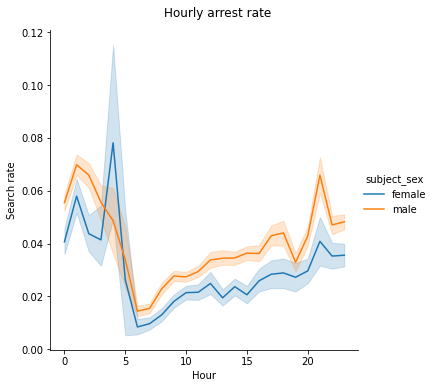
\includegraphics[scale=0.34, valign=t]{../figures/fig_arrest_day.png}}
\subfloat[]{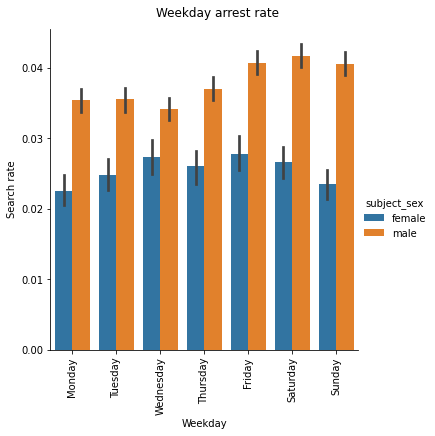
\includegraphics[scale=0.34, valign=t]{../figures/fig_arrest_weekday.png}}
\subfloat[]{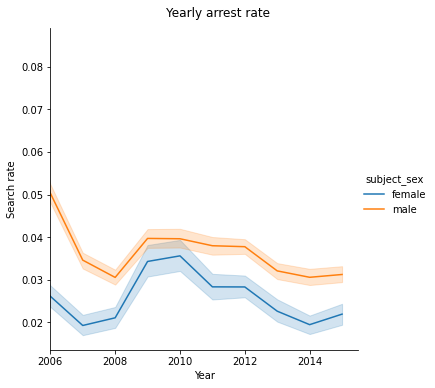
\includegraphics[scale=0.34, valign=t]{../figures/fig_arrest_year.png}}
\caption{Search rate as a function of: hour in the day (a), weekday (b) and year (c) split by the gender of the conductor.} \label{fig:time_studies}
\end{figure}   
\FloatBarrier

Figure~\ref{fig:time_studies} (a) shows the search rate as a function of the hour in the day. We see that most of the searches occur at night time, between 9 pm and 5 am. 

Figure~\ref{fig:time_studies} (b) shows the search rate as a function of the week of the day. The distribution for females looks rather flat while for males there is a slight increase of searches during the weekends, from Friday to Sunday.

 Figure~\ref{fig:time_studies} (c) shows the search rate by years. We observe a mild decrease in the search rate over the years after 2010. Figure~\ref{fig:arrest_search} shows that the decrease in the search rates translates into a decrease in the arrest rate as well. 

 \begin{figure}[h]
 \centering
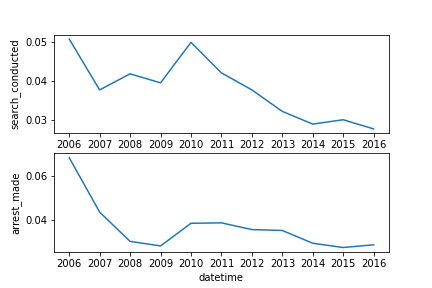
\includegraphics[scale=0.4, valign=t]{../figures/arrest_search.png}
\caption{Comparison of search and arrest rates over time.} \label{fig:arrest_search}
\end{figure}   
\FloatBarrier


\section{Studies by district}

The dataset provides information about the district where the stop happened. We look at the reasons for stop in each of the different districts. This is shown in Figure~\ref{fig:district}. District X1 has significantly less stops that the rest of the districts. In the K districts the stops due to speeding are the most common ones. This also true in the X districts, however, in those the gap with respect to the other reasons is not as big. 

 \begin{figure}[h]
 \centering
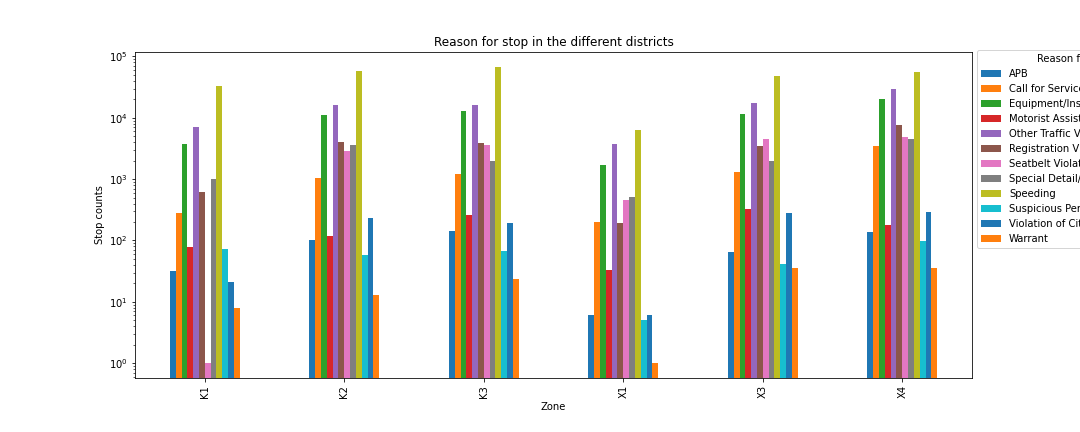
\includegraphics[scale=0.4, valign=t]{../figures/fig_violations_district.png}
\caption{Reason for the stop in the different districts.} \label{fig:district}
\end{figure}   
\FloatBarrier

\section{Adding weather data}
We now use weather data from a different dataset to understand if weather conditions affect the police stops. For that, we use weather data from the National Center for Environmental Information collected at the Rhode Island weather station, USW00014765~\cite{WeatherWeb,WeatherWeb1}\footnote{This is meant as an exercise and we understand that weather data from a single weather station is not representative for the data in the whole state}. We subset the dataset to keep only data from 2005 to 2019.

The weather dataset contains 20 columns that start with 'WT', each of which represents a bad weather condition. For example:

\begin{itemize}
\item WT05 indicates "Hail"
\item WT11 indicates "High or damaging winds"
\item WT17 indicates "Freezing rain"
\end{itemize}

For every row in the dataset, each WT column contains either a 1 (meaning the condition was present that day) or NaN (meaning the condition was not present).

We quantify "how bad" the weather was each day by counting the number of 1 values in each row. This is depicted in Figure~\ref{fig:weather}. There is a peak at 0, which means that most of the times there is good weather. The counting of bad weather conditions ranges from 0 to 9. We use this information to create a "bad weather rating" as follows:

 \begin{figure}[h]
 \centering
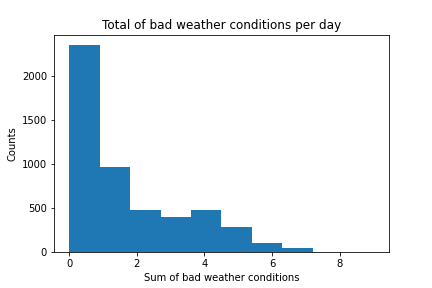
\includegraphics[scale=0.5, valign=t]{../figures/fig_bad_weather_conditions.png}
\caption{Distribution of bad weather conditions.} \label{fig:weather}
\end{figure} 

\begin{itemize}
\item Convert 0 to 'good'
\item Convert 1 through 4 to 'bad'
\item Convert 5 through 9 to 'worse'
\end{itemize}

According to this categorisation, the distribution of the weather conditions looks as in Figure~\ref{fig:weather_rating}. There is an equal number of days with good and bad weather, while there are few days where the weather was worse.

 \begin{figure}[h]
 \centering
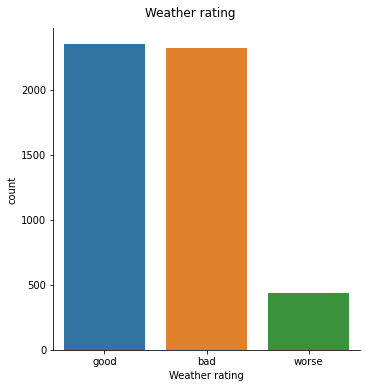
\includegraphics[scale=0.4, valign=t]{../figures/weather_rating.png}
\caption{Distribution of weather rating.} \label{fig:weather_rating}
\end{figure} 
  
We now merge the two datasets to compare the police stops to the weather conditions. Figure~\ref{fig:weather_arrest_reason} shows the frequency of arrests made as a function of the reason for the stop and the weather rating. 

 \begin{figure}[h]
 \centering
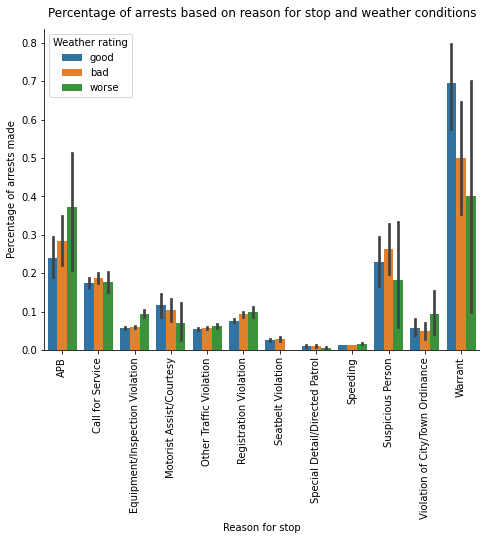
\includegraphics[scale=0.7, valign=t]{../figures/fig_arrest_reason_weather.png}
\caption{Frequency of arrests made as a function of the reason for the stop and the weather rating.} \label{fig:weather_arrest_reason}
\end{figure} 


\FloatBarrier
\newpage
\bibliographystyle{plain} 
\bibliography{references}

\end{document}
